\documentclass[a4paper,10pt]{article}
\usepackage[utf8]{inputenc}
\usepackage[brazilian]{babel}
\usepackage{graphicx}        % standard LaTeX graphics tool
\usepackage{color,enumerate}
\usepackage{subfigure}
\usepackage{tikz}
\usepackage{fullpage,amsmath,amssymb}
\title{2022-1: Lista de exercícios 01}
\author{Ronaldo de Freitas Zampolo}

\begin{document}
Universidade Federal do Pará

Instituto de Tecnologia

Faculdade de Engenharia da Computação e Telecomunicações

EC01045 - Processamento digital de sinais

Prof. Ronaldo de Freitas Zampolo

\begin{center} \textsc{2022-2: Lista de exercícios 01} \end{center}

%\maketitle
\begin{enumerate}
	\item Seja um sistema discreto LI (linear e invariante), cuja resposta ao impulso é 
		\begin{equation*}
			h[n] = \delta[n] + \delta[n-1]
		\end{equation*}
		\begin{enumerate}
			\item Determine a resposta em frequência deste sistema $H(e^{j\omega})$, se possível.
			\item Calcule a função de transferência $H(z)$.
			\item Esboce o diagrama de pólos e zeros, indicando também a região de convergência.
			\item Que tipo de sistema é esse? Marque a resposta correta e justifique sua resposta.
				\begin{enumerate}
					\item Passa-baixas
					\item Passa-altas
					\item Passa-banda
					\item Rejeita-banda
				\end{enumerate}
			\item A resposta ao impulso desse sistema é do tipo:
				\begin{enumerate}
					\item FIR
					\item IIR, à direita
					\item IIR, à esquerda
					\item IIR, bilateral
				\end{enumerate}
				Marque e justifique sua resposta.
			\item O sistema é estável? Justifique sua resposta usando a região de convergência de $H(z)$.
			\item Ache a equação de diferenças para o sistema.
		\end{enumerate}
	\item Um sistema LI tem resposta ao impulso dada pelo gráfico
		\begin{figure*}
			\centering
			%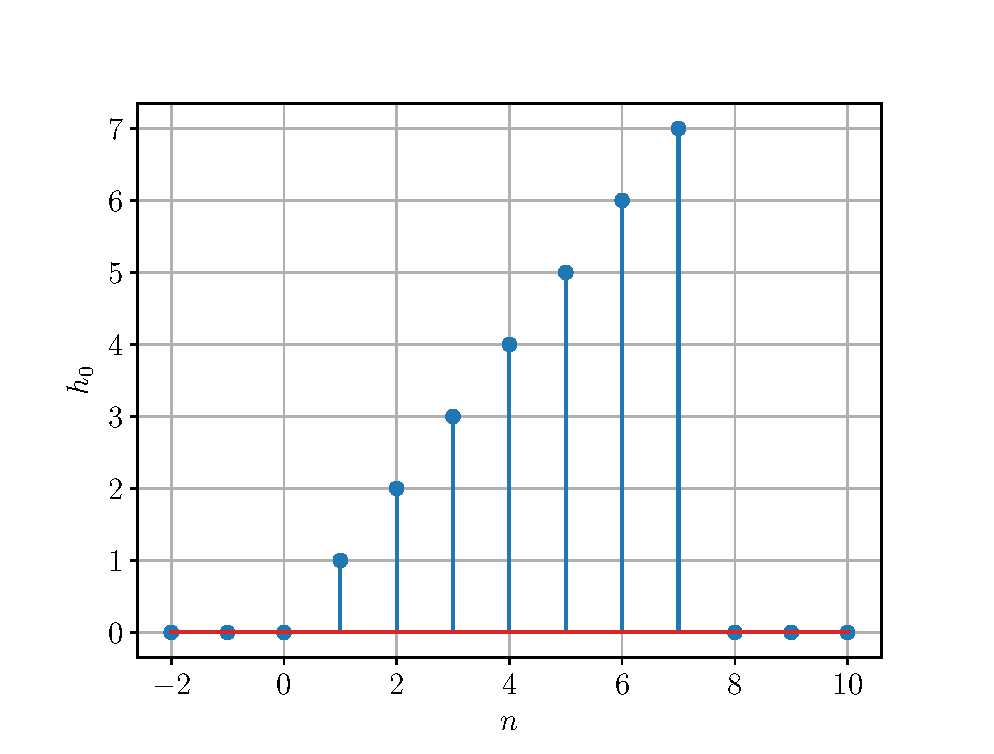
\includegraphics[width=0.5\textwidth]{figs/h0}
			\label{fig:h0}
			\caption{Resposta ao impulso}
		\end{figure*}
		\begin{enumerate}
			\item Qual a função de transferência $H_0(z)$ do sistema? Calcule pólos e zeros, e indique-os no plano complexo Z.
			\item Suponha que $H_1(z) = H_0(z)$. Determine os pólos e zeros de $H_1(z)$, indicando-os no plano complexo Z.
			\item Determine $h_1[n]$.
		\end{enumerate}
\end{enumerate}
\end{document}
